
\section{Organisation of Data Management} \label{sec:org}

The Organisation and management of DM is covered in detail in \cite{LDM-294}.
As shown in \figref{fig:org} DM Management is aligned mainly along the Work Breakdown Structure (WBS) of the project.
It was found that a strict adherence to the WBS structure led to some products not being the responsibility's of a single manager when they spanned the organisation.
To address this two cross cutting teams were identified  to take care of the Science Platform and middleware.
Each of these areas was then assigned to a manager to ensure its delivery - these managers were requested resources across the subsystem as needed.

Also of note in \figref{fig:org} are the product owners.
To ensure a single voice toward developers the product owner interprets requirements and sets priorities for the
project.
This also involves being the point of contact for any other stakeholders and incorporating their needs or wishes in the system.
Interpretation of requirements is always difficult on large projects like Rubin observatory, they exist over a long period of time, were often written by people no longer on the project, and frequently are not easily verifiable.
Hence another important roll of the product owner is in defining the verification tests for the requirements.
Tests give a very concrete interpretation of the requirement.
Verification covers all subsystems, software and data  see \cite{PSTN-024}.
  DM will be verified and validated as part of System verification and validation \cite{2014SPIE.9150E..0NS} \cite {PSTN-029}



\begin{figure}
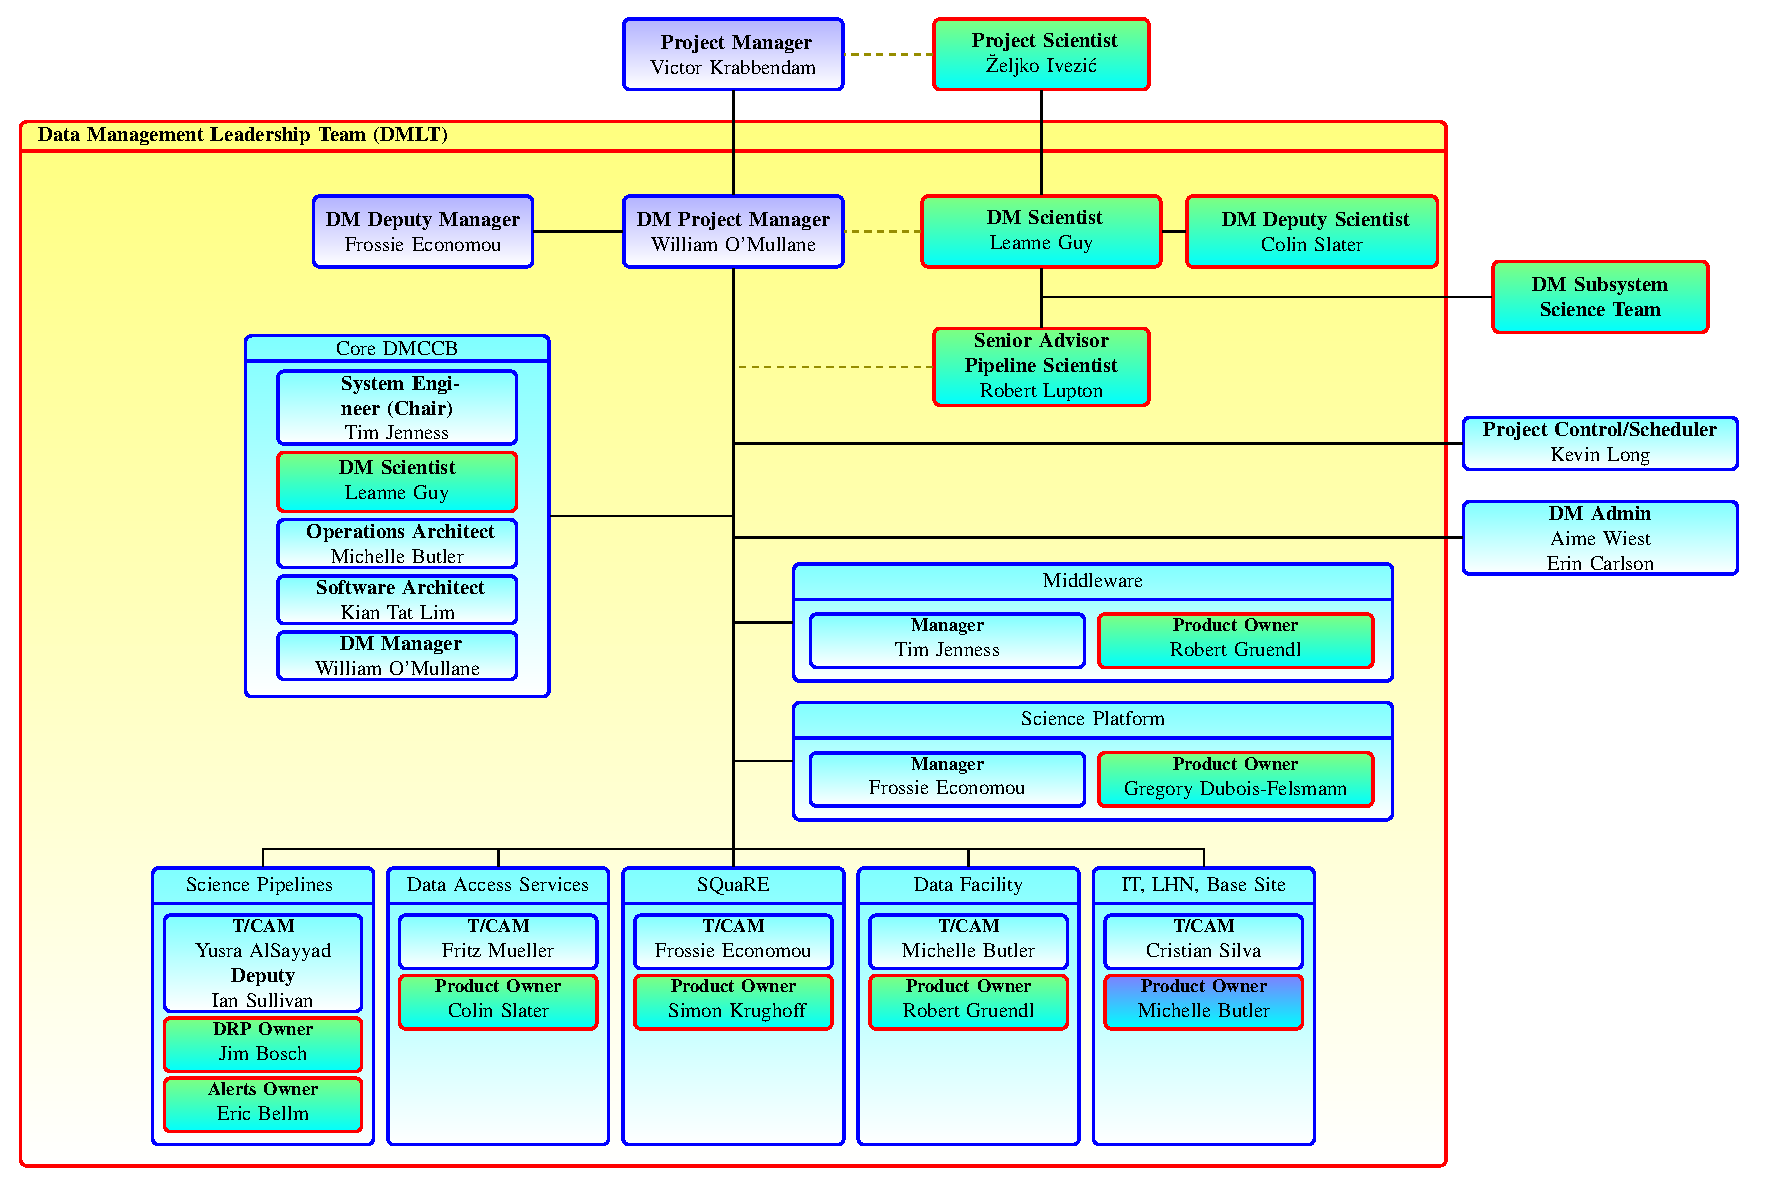
\includegraphics[width=0.9\textwidth]{images/DmOrg}
	\caption{Org chart for Rubin DM from \cite{LDM-294}\label{fig:org}}
\end{figure}

\subsection{Open development process}\label{sec:devproc}
From the outset DM was seen as a large scientific  software project.
Agile methodologies \cite{it:agile}  are particularly suited to the uncertainties of a science project and
a cyclical approach to software development, with a period of six months was adopted early on.
A set of Epics corresponding to major pieces of work are defined at the beginning of each cycle.
Tickets to track the work are created in Jira.

All code, and in fact documents, are kept under continuous integration using a mixture of Jenkins and GitHub Actions.
Everything it under an open source licensed (mainly GPL) and available openly on GitHub.com.
For the pipelines traditional releases are made each six months.
Within SQuaRE services are released as needed and continuously deployed (currently with ArgoCD).

This is a large NSF funded project and so must still adhere to a more waterfall style of reporting.
Milestones for major functionality, tied to major project milestones, were laid out and tracked in the usual manner.
The DM approach to the Earned Value Management System (EVMS) used through Rubin construction is shown in \cite {DMTN-020}.

\subsection{Mode of work}\label{sec:mode}
The DM  team is distributed in several centers across the continental US as well as Chile and France.
A strong set of guidelines \href{https:\\developer.lsst.io}{developer.lsst.io} was introduced early on to help homogenize modes of work e.g. dealing with tickets, naming github branches, merges, code style etc.
It has functioned as a distributed organisation from the beginning, which probably help it weather the COVID-19 pandemic reasonably well.
The Technical Account Managers (T/CAM), as shown in \figref{fig:org}, have a large degree of autonomy to deliver their software products.
The Data Management Leadership Team (DMLT) comprises the managers and product owners and has a brief (30 minute) weekly meeting to set direction and raise issues (on Mondays).
There is a longer multi day meeting three or four times a year some of which were physical get togethers, at least before the pandemic.
The Managers have a standup meeting on Thursdays to work out any blockages or anticipated issues between the teams.
Each team has its own regular meetings and discussions.

There is a mature decision making process where, in general, decisions are made at the lowest level possible within the team i.e. at the level of the individual developer where practical. This is enshrined the \href{https://developer.lsst.io/team/empowerment.html}{empowerment section of the guide}.
When this is not possible, decision making is escalated through the hierarchy using  the \href{https://developer.lsst.io/communications/rfc.html}{Request for Comments (RFC) mechanism}.
DM captures decision making in technical notes (the DMTN series) or formal documents (the LDM series).


\subsection{Relationship to other subsystems}

As already mentioned all of Rubin interacts with System Engineering
   We take images from the  LSST camera: \cite{2010SPIE.7735E..0JK}

   We are commanded and listen to the  Telescope  and site software  \cite{2014SPIE.9145E..1AG}


